\section{Composition "Music for multilayered temporal structures"}

This composition consists primarily of two components: "Etudes" composed using the aforementioned "music for multilayered temporal structures" method, and "performance instructions" for playing these pieces. The compositions here are notated in the so-called "lead sheet" format. Figure \ref{fig:figure_09} shows the lead sheet for "All the Things You Are" from "The Real Book 5th Edition."

\begin{figure}[H]
\centerline{
	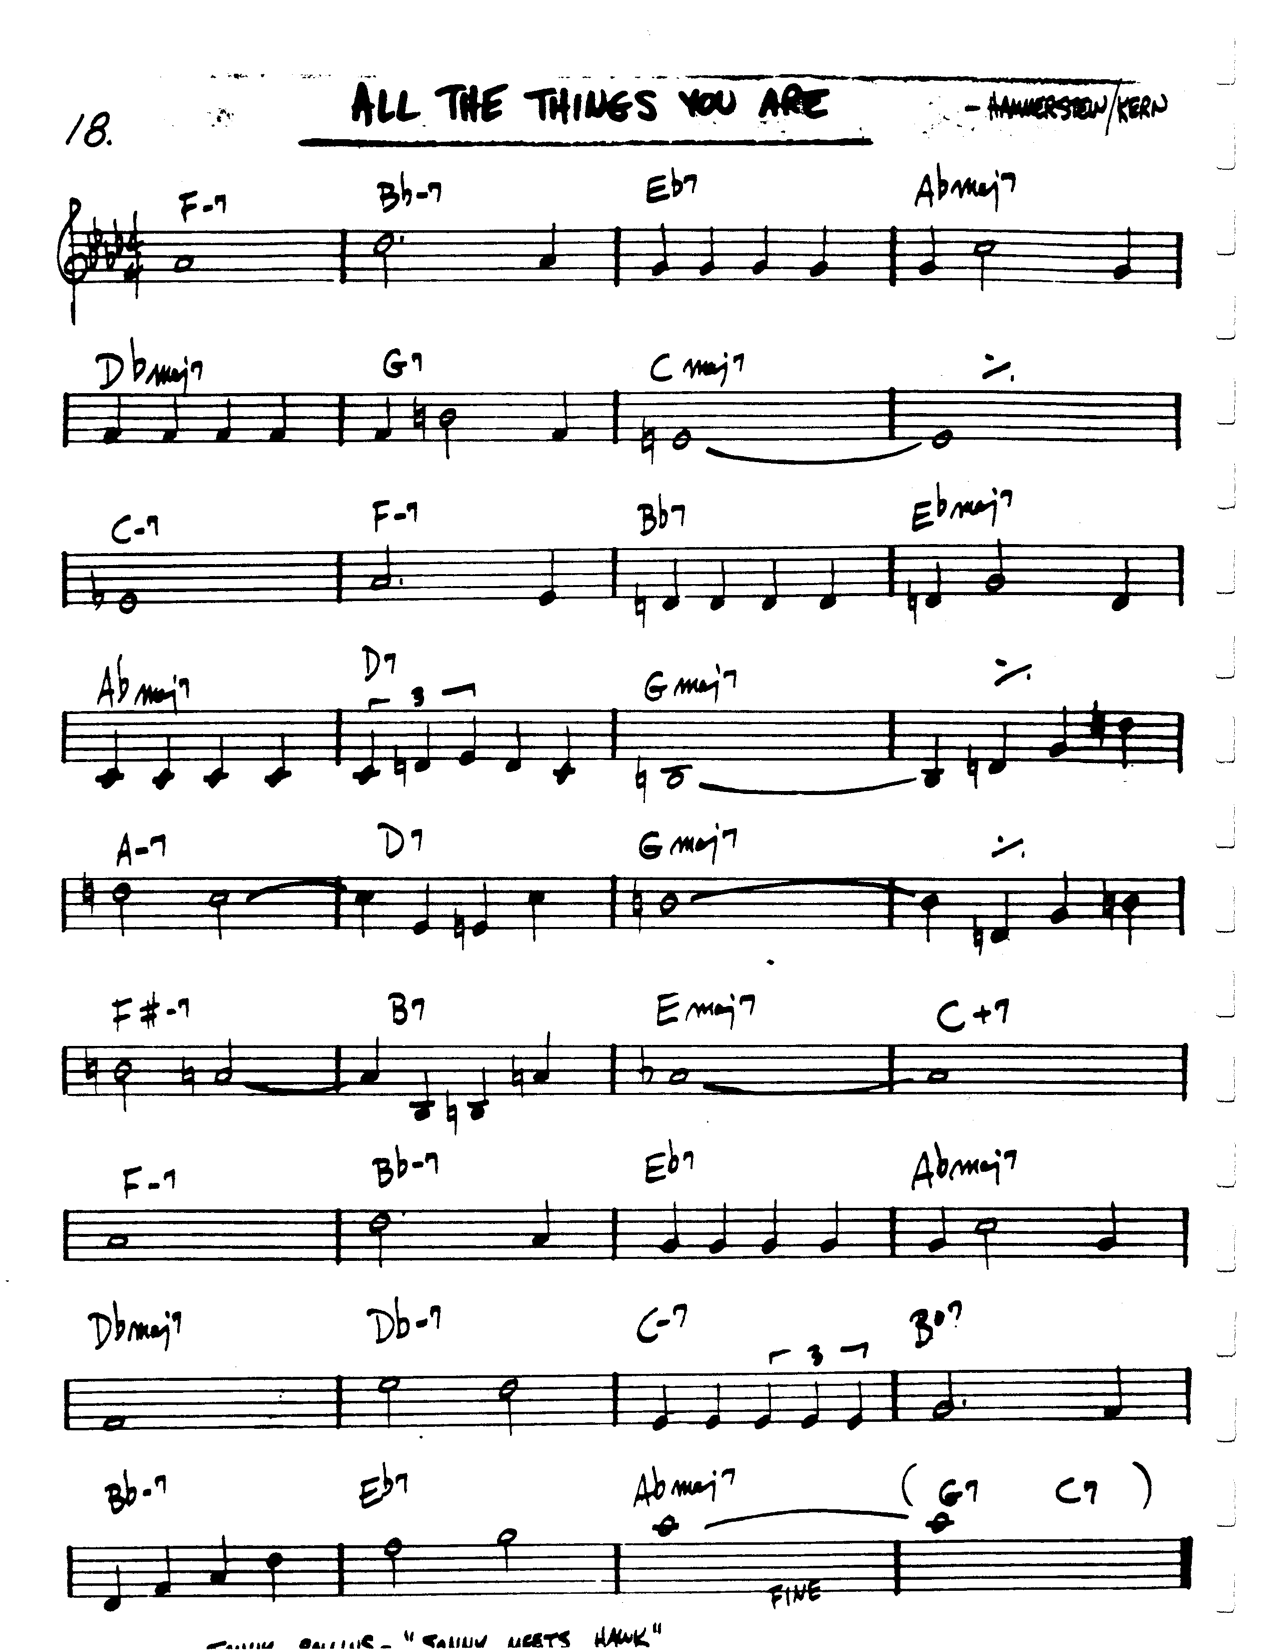
\includegraphics[
 width=0.5\textwidth]{./PDF/figure_09.pdf}
}
\caption{"All the Things You Are" lead sheet}
\label{fig:figure_09}
\end{figure}

Such lead sheets are meta-descriptive musical scores that indicate the structure of a piece through elements such as "key," "time signature," "melody," and "chord progression." They represent one of the notational formats widely utilized in jazz and popular music, as exemplified by The Real Book. For this work, I adopted the lead sheet format as a method for establishing the piece as popular music. Furthermore, by adopting lead sheets and questioning the reproducibility of the basic popular music format—instrumental ensemble—I considered this approach effective for contemplating the future physicality of music from the historical background inherent in lead sheets.

\subsection{Positioning of Lead Sheets and Composition Concept}

After "{\bf Berliner invented the disc-type recording medium in 1885}" \cite{murai:01}, "{\bf radio broadcasting that began in 1920 spread across the United States in a short period, and by 1924, there were over 1,200 broadcasting stations throughout America}" \cite{murai:01}. However, regarding music distribution prior to this, Murai states: "{\bf 'Home Sweet Home' was (omitted) published in 1823 and became a huge hit, selling millions of copies of sheet music. (omitted) Hits were based on sheet music sales}" \cite{murai:01}. This indicates that sheet music was "{\bf the first commercialized popular music, predating records}" \cite{kikuchi-ootani:01}. Additionally, in the essay "On Schillinger and Berklee Theory" by Jun'ichi Ishizuka, published in "The School That Taught Melancholy and Sensuality," the period following the emergence of the Berklee School of Music (later College of Music) and the Berklee Method in 1954 is described as follows:\\

{\bf In other words, the Berklee Method is a thoroughly structured system that reinterprets the blues through classical harmony theory and aligns it with the new concept of chords. (omitted) Classical music theory is also digested in a form suitable for popular music practice. (omitted) And it must not be forgotten that what supported this new method was none other than the development of recording technology. Recording technology rescued improvised music—which lacked detailed notation and would otherwise dissipate after a single performance—from oblivion. It became possible to play back recordings repeatedly, broadcast them, and create a global market by pressing tens of thousands of records. This dismantled the absolute superiority of classical music based on notation and laid the groundwork for music based on loose theoretical systems like the Berklee Method to dominate the world. Theory generalized through recording technology. Due to this origin, it became inseparable from technological issues represented by the recording technology of subsequent popular music.}\\

What Ishizuka refers to as "improvised music without detailed notation" clearly indicates jazz as popular music of that era. Furthermore, the Berklee Method exists as a commonly used music theory in the contemporary development of jazz. In this context, this work targets "The Real Book," a collection of lead sheets. As previously mentioned, lead sheets indicate the structure of a piece through "key," "time signature," "melody," and "chord progression." This is, as Ishizuka points out, "thoroughly structured in a form suitable for the new concept of chords." This structuring can be understood by listening to performances by various musicians of "All the Things You Are," as shown in the lead sheet in Figure \ref{fig:figure_09}. However, what guarantees that "this piece is 'All the Things You Are'" is the structural consistency shown in the lead sheet, not the exact reproduction of phonetics or tuning. This becomes clear in actual performance: "no two performances are the same, yet all are recognized as the same piece." This can be rephrased as follows:\\

{\bf A lead sheet is: diversity of expression due to differences in physicality + guaranteed reproducibility through structural consistency = a score as meta-composition}\\

Therefore, I targeted the positioning of lead sheets as scores for meta-composition and The Real Book as a so-called "collection of standards" using lead sheets. By employing lead sheets in the work, I aimed to ensure the relationship between music and the body as popular music while making it possible to consider the next relationship between music and the body, establishing the concept "Beyond The Real Book" within the work.

\subsection{Work Structure}

This work consists of the following content:

\begin{enumerate}
  \item Explanation of the composition concept
  \item Explanation of "music for multilayered temporal structures"
	\item "Etude \#1" performance instructions
	\item "Etude \#1" lead sheet
	\item "Etude \#2" performance instructions
	\item "Etude \#2" lead sheet
	\item "Etude \#3" performance instructions
	\item "Etude \#3" lead sheet
\end{enumerate}

This is written with the purpose of having performers read each instruction document and master the ensemble of "music for multilayered temporal structures." Each etude is composed with specific learning objectives and is designed to facilitate performers' gradual acquisition of skills.

\subsection{Compositional Intent and Relationships Between Each Etude}

Both "Etude \#1" and "Etude \#2" consist of two layers: "4 beats in 4/4 time" and "5 beats in 4/4 time." In "Etude \#1," the melody plays "4 beats in 4/4 time" while the bass plays "5 beats in 4/4 time." The rhythm patterns for drums are organized with the intention of explicitly indicating the characteristic pulse points of both time signatures. Therefore, the performer playing the melody can generate their own pulse from the "4 beats in 4/4 time" indicated by the drummer, and similarly, the performer playing the bass part can feel the "5 beats in 4/4 time" from the drummer and generate their pulse. However, the "5 beats in 4/4 time" in the bass part intentionally omits the first beat, requiring more accurate sensing of the pulse in the empty spaces. Such devices were employed because the purpose of this etude is "acquiring fundamental skills in music for multilayered temporal structures." Additionally, being a one-mode piece in D Dorian makes it difficult to feel the harmonic rhythm, which is also intentionally aligned with the aforementioned purpose. Figure \ref{fig:figure_11} shows the lead sheet for "Etude \#1."

\begin{figure}[htb]
\centerline{
	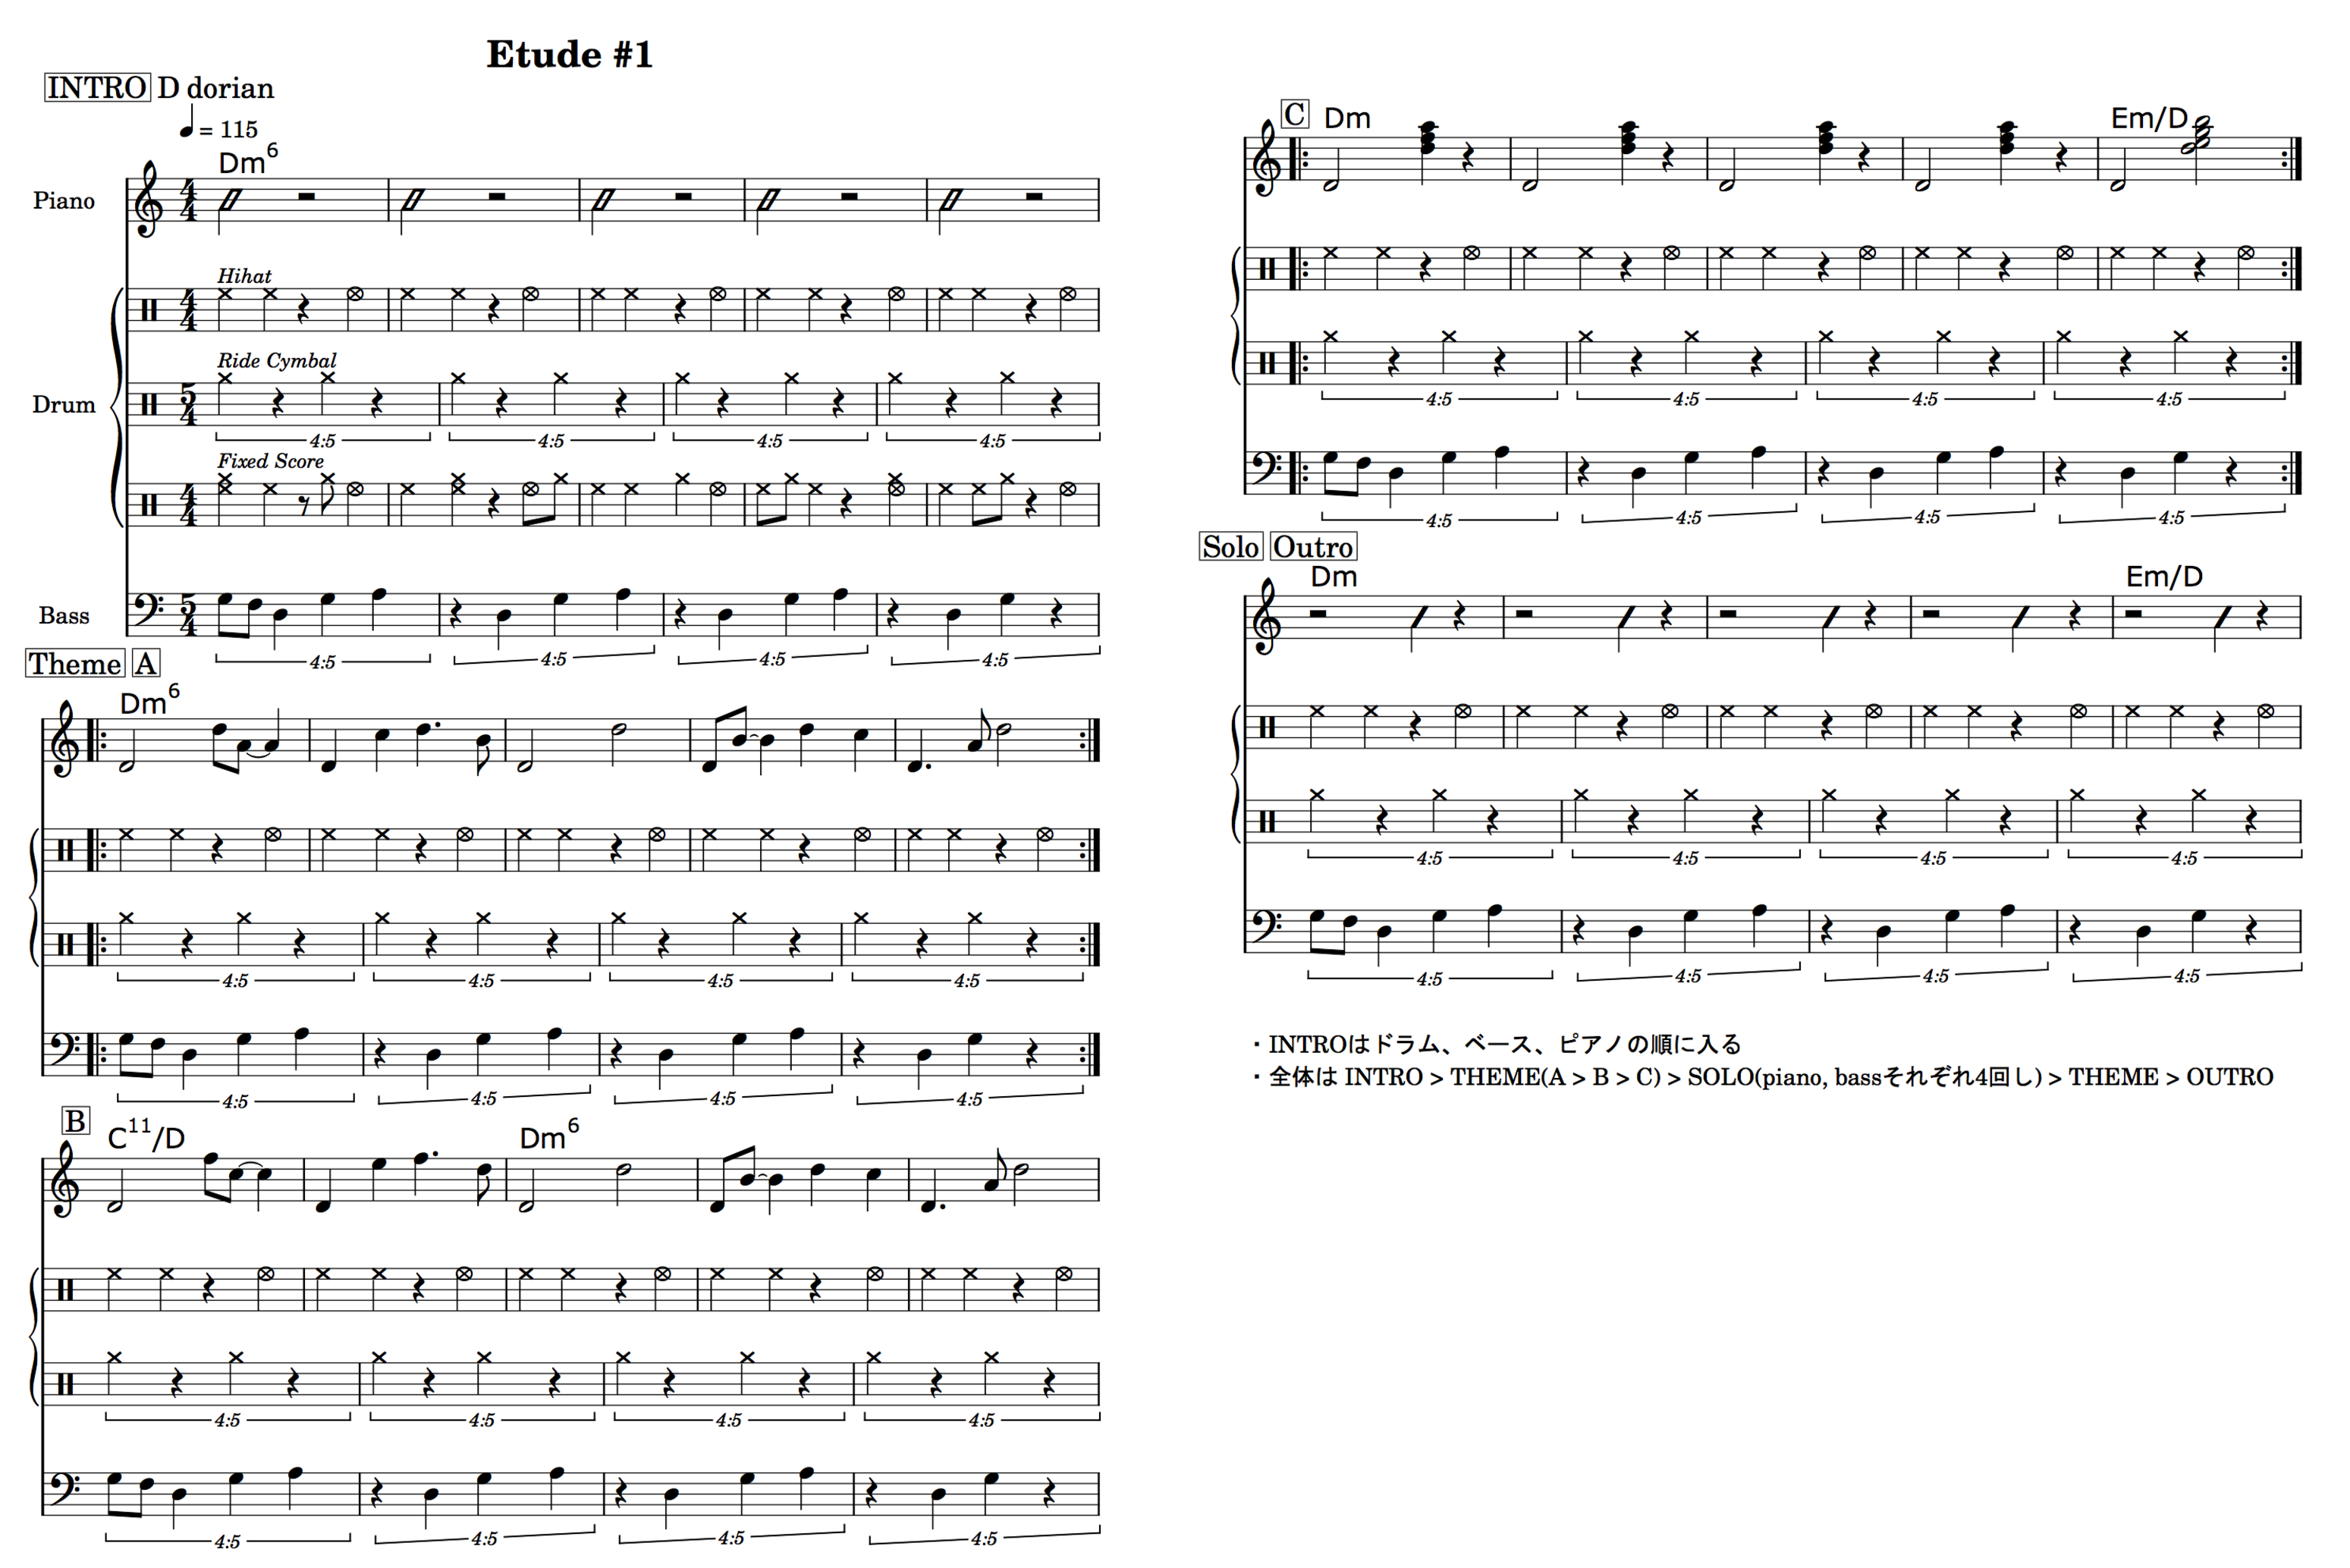
\includegraphics[
 width=\textwidth]{./PDF/figure_11.pdf}
}
\caption{"Etude \#1" lead sheet}
\label{fig:figure_11}
\end{figure}

"Etude \#2" features chord progressions compared to "Etude \#1," making the harmonic rhythm easier to feel, and the piece follows the commonly seen AABA form. However, in the B section, the melody and bass exchange their respective time signatures. Additionally, the explicit indication of rhythm by drums is reduced, requiring performers to generate the pulse of each time signature through mutual structural understanding, as shown in Figure \ref{fig:figure_07}. This piece has the objective of "acquiring application of music for multilayered temporal structures and rhythm exchange," and the composition was created with this intention. Figure \ref{fig:figure_12} shows the lead sheet for "Etude \#2."

\begin{figure}[htb]
\centerline{
	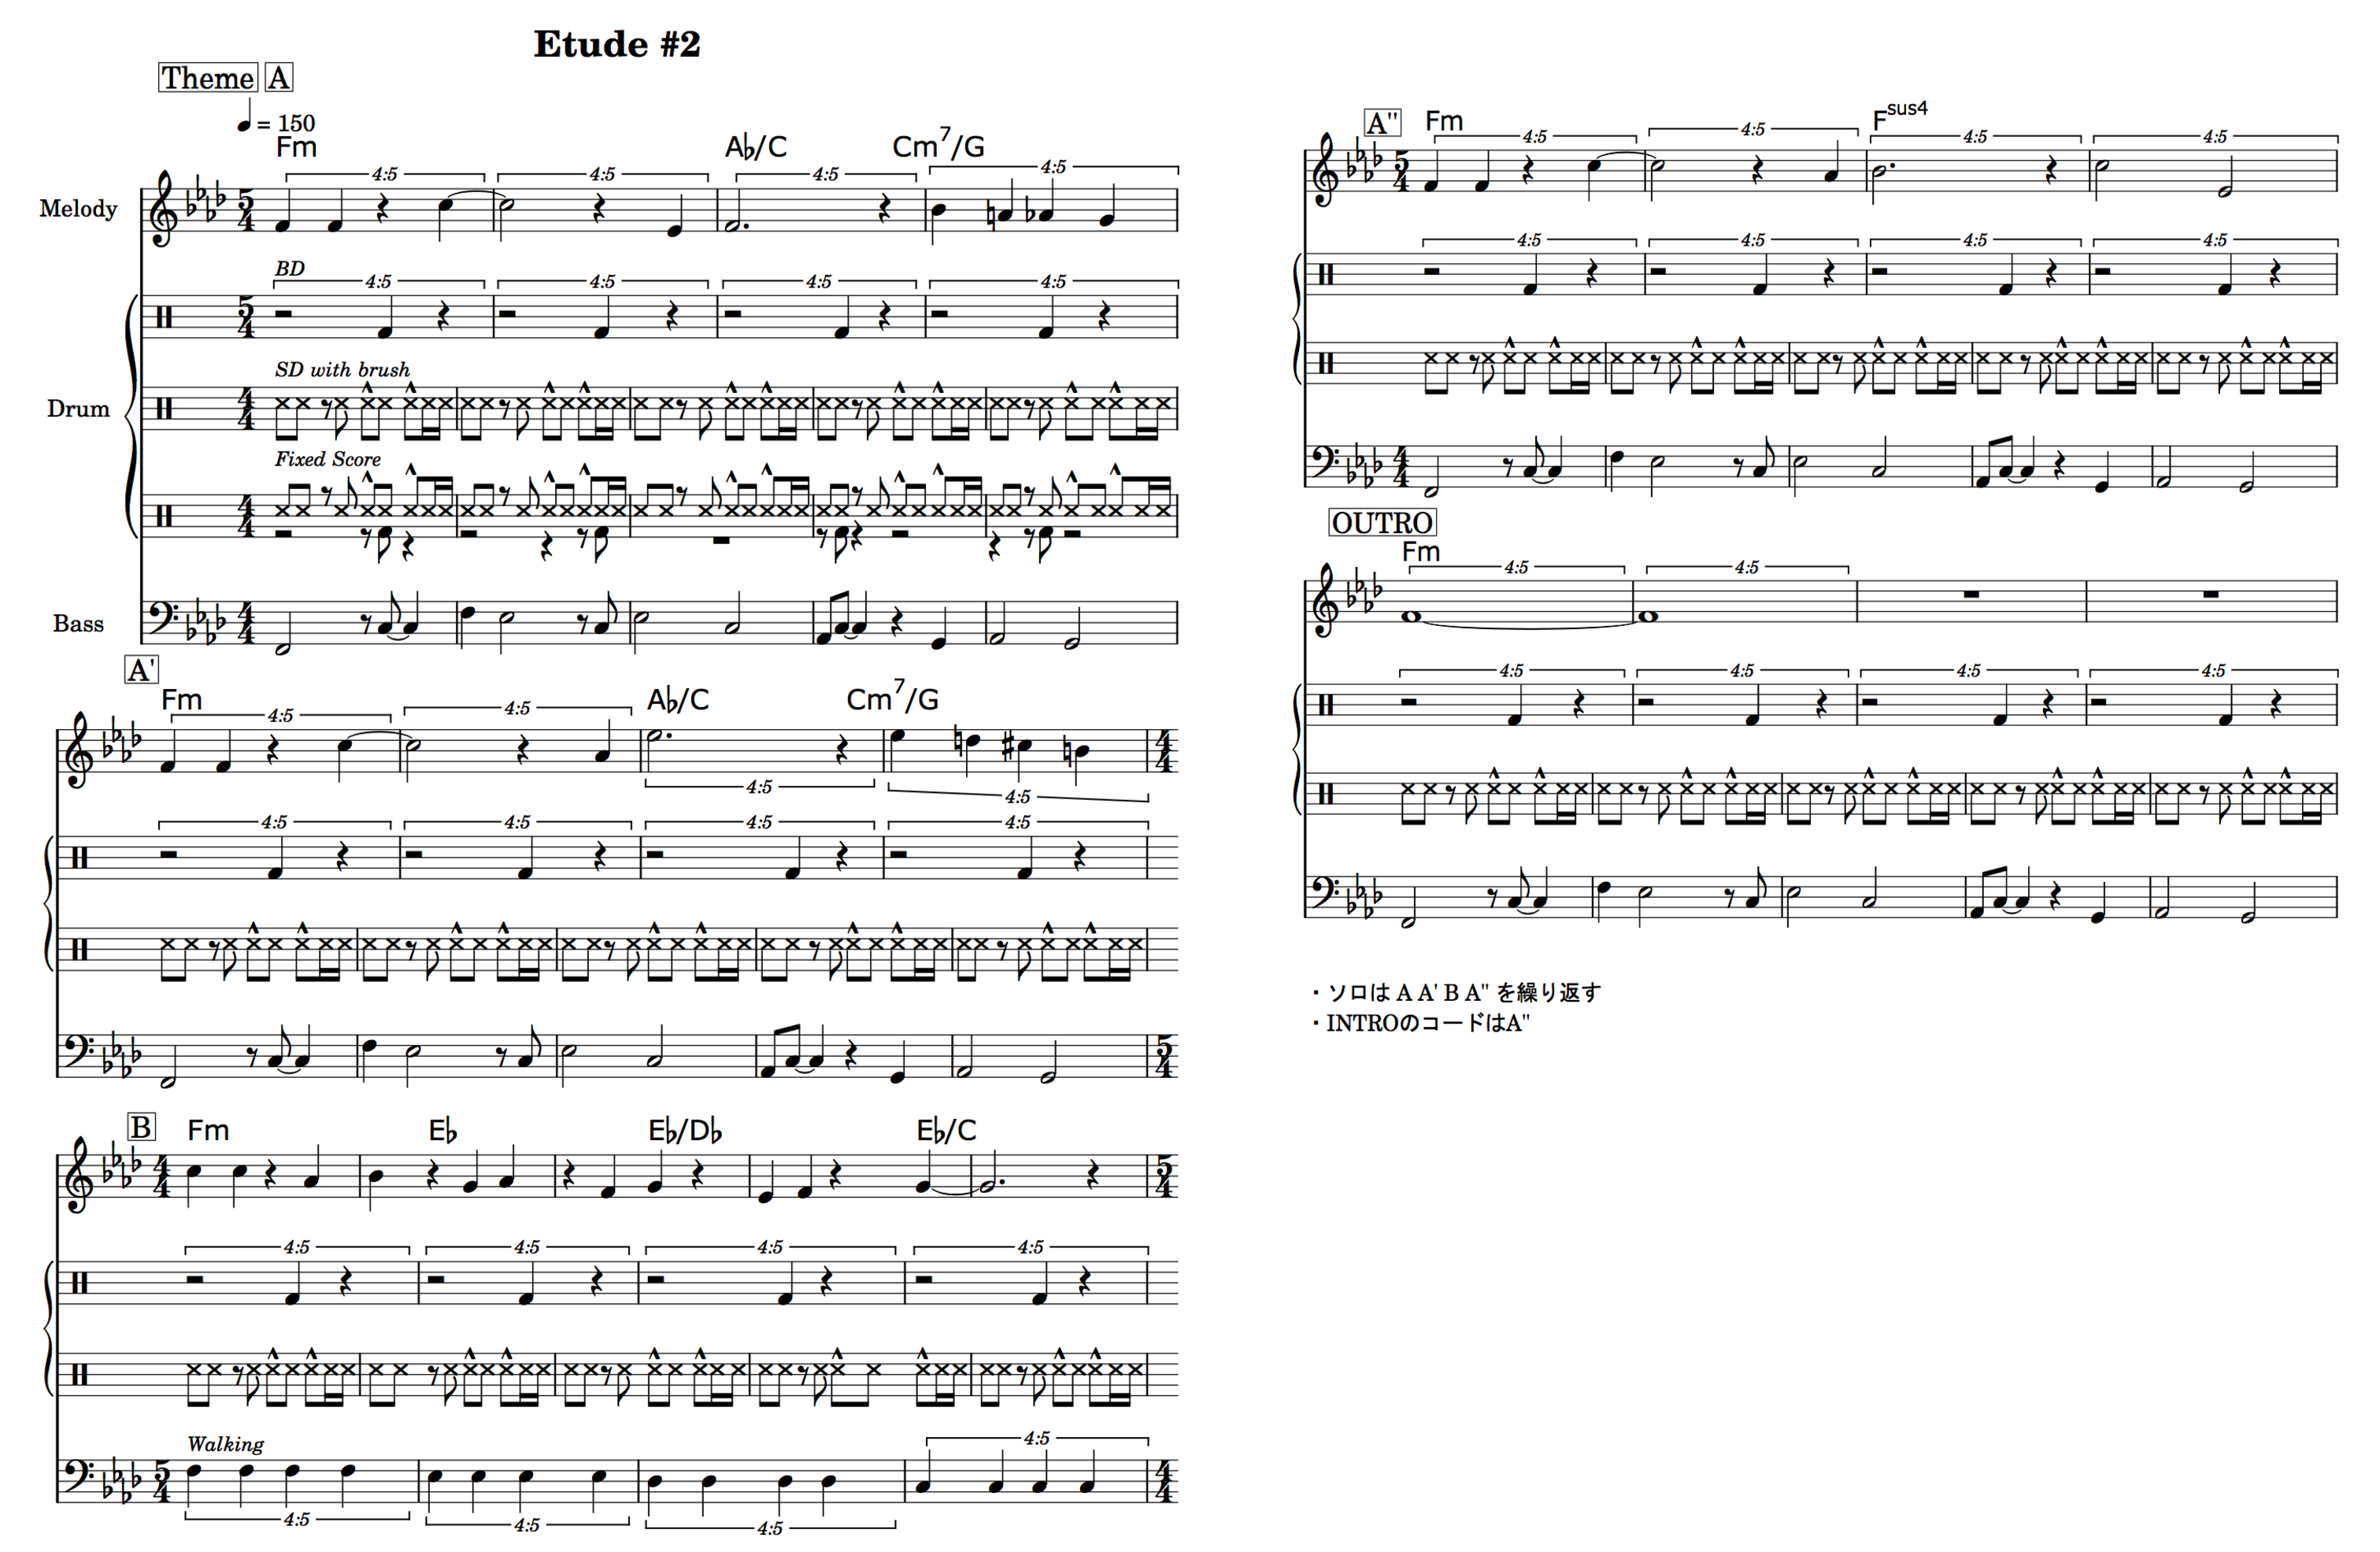
\includegraphics[
 width=\textwidth]{./PDF/figure_12.pdf}
}
\caption{"Etude \#2" lead sheet}
\label{fig:figure_12}
\end{figure}

"Etude \#3" distinguishes itself musically from "Etude \#1" and "Etude \#2" and increases difficulty by being composed in three layers: "3 beats in 4/4 time," "4 beats in 4/4 time," and "5 beats in 4/4 time." A significant feature is that this piece does not provide the drum assistance for each time signature seen in "Etude \#1" and "Etude \#2." Therefore, as shown in Figure \ref{fig:figure_07} for "Etude \#2," each performer must structurally understand their pulse from the piece and perform accordingly. Additionally, this piece features circular chord progressions, demonstrating "the potential for polytonality inherent in music for multilayered temporal structures." Figure \ref{fig:figure_13} shows the lead sheet for "Etude \#3." Each lead sheet can also be viewed in the work "Music for multilayered temporal structures" \cite{yamato:01}. The work can be downloaded from the following URL: \url{https://goo.gl/o1pTEk}

\begin{figure}[H]
\centerline{
	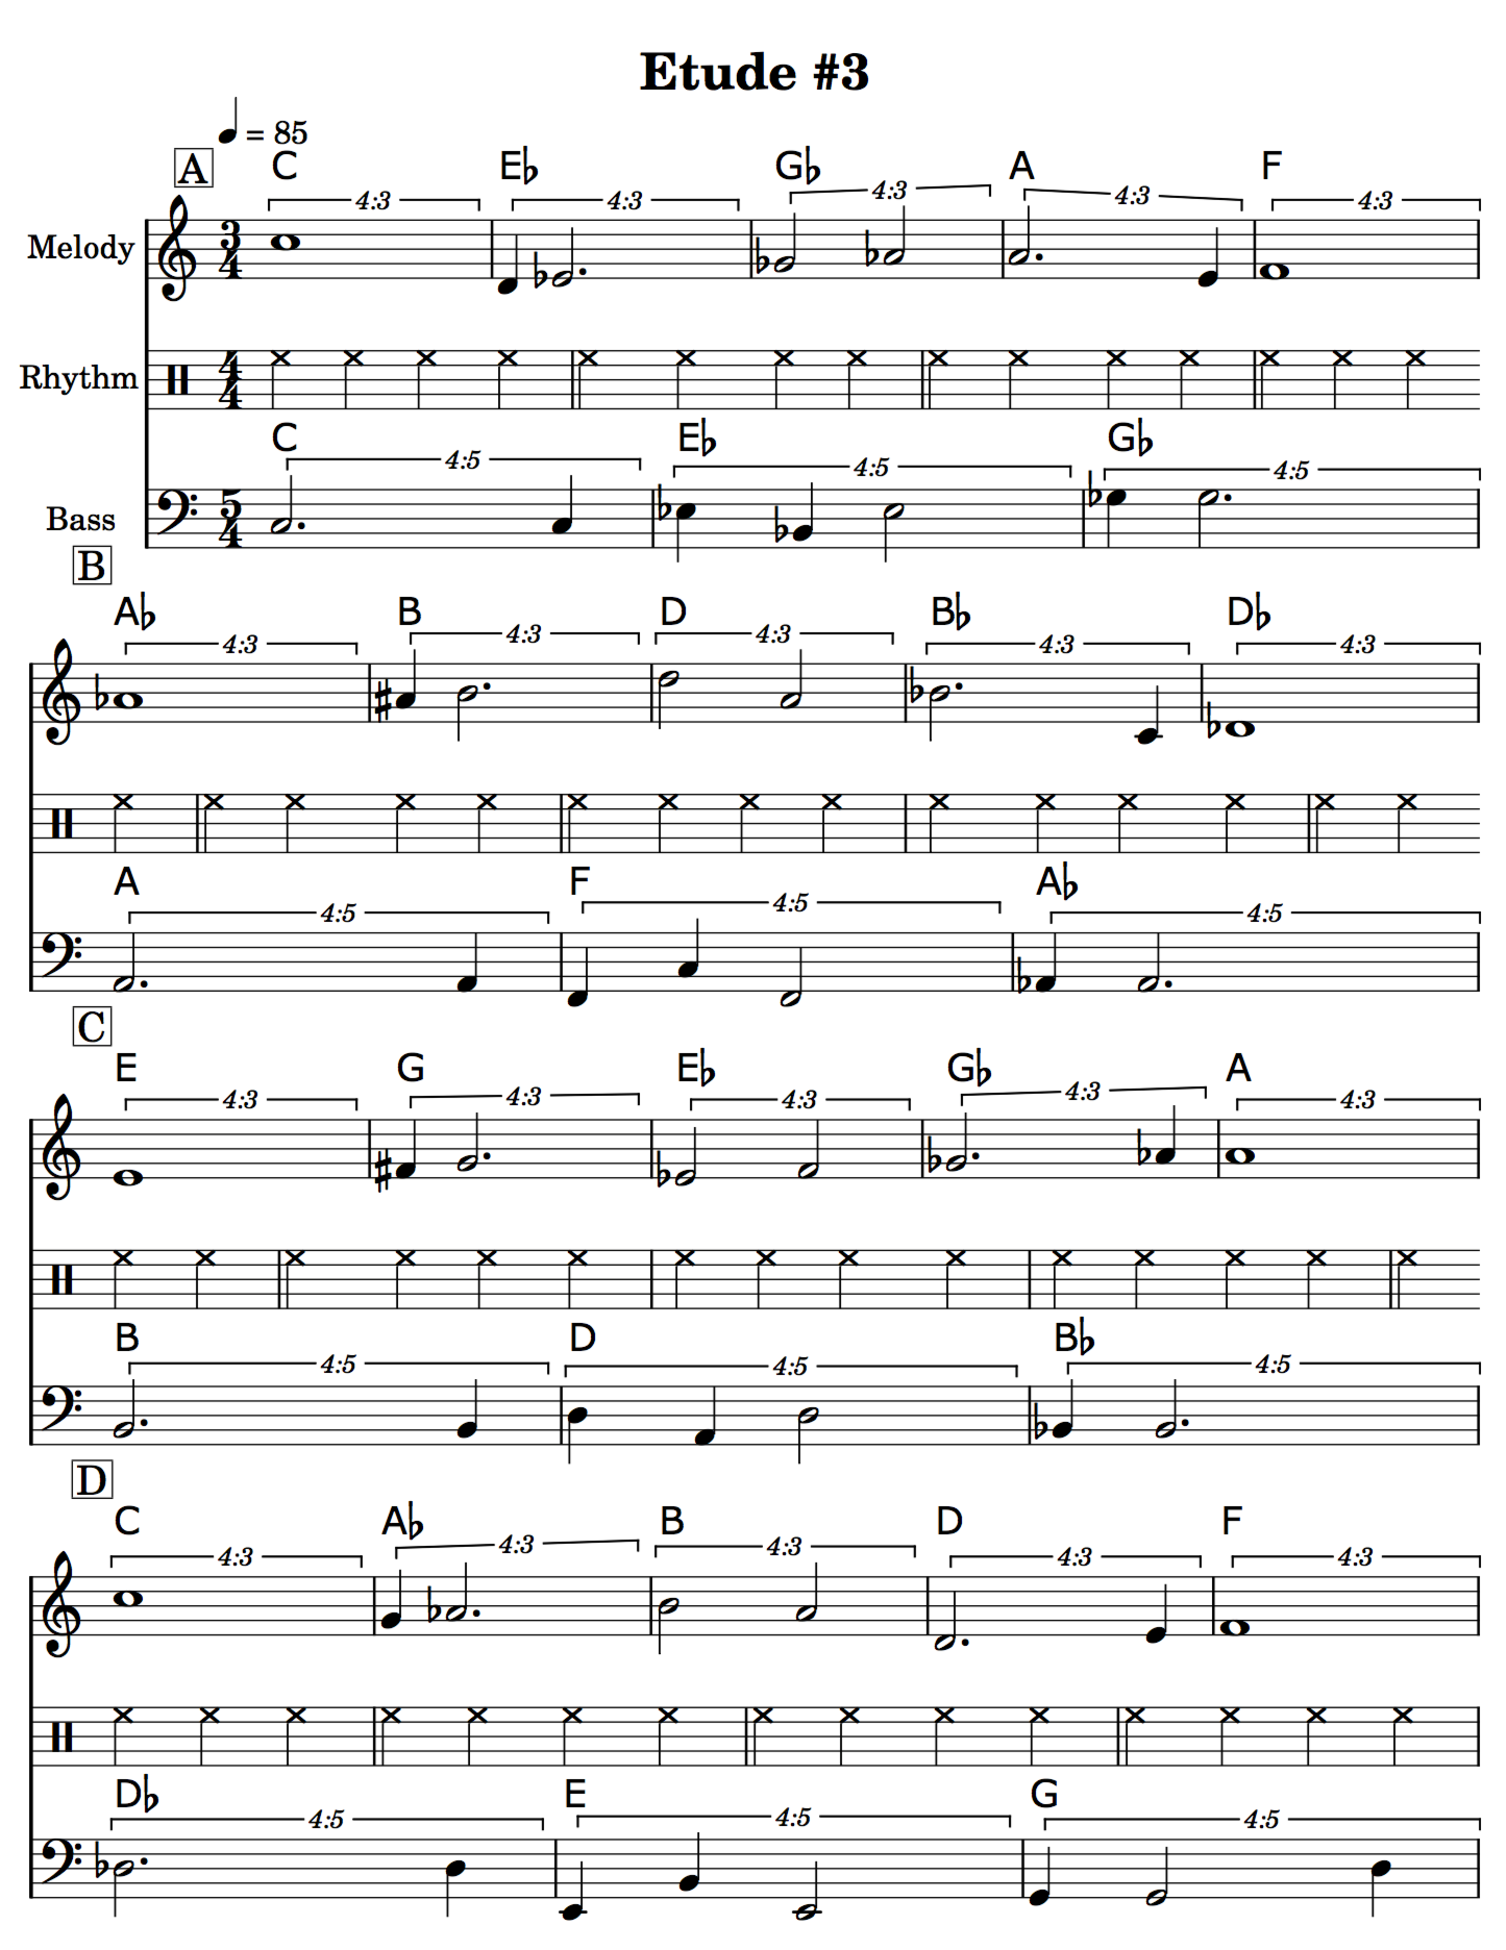
\includegraphics[
 width=0.5\textwidth]{./PDF/figure_13.pdf}
}
\caption{"Etude \#3" lead sheet}
\label{fig:figure_13}
\end{figure}

Summarizing the relationships between the above etudes, as shown in Figure \ref{fig:figure_10}, the difficulty gradually increases from 1 to 3.

\begin{figure}[H]
\centerline{
	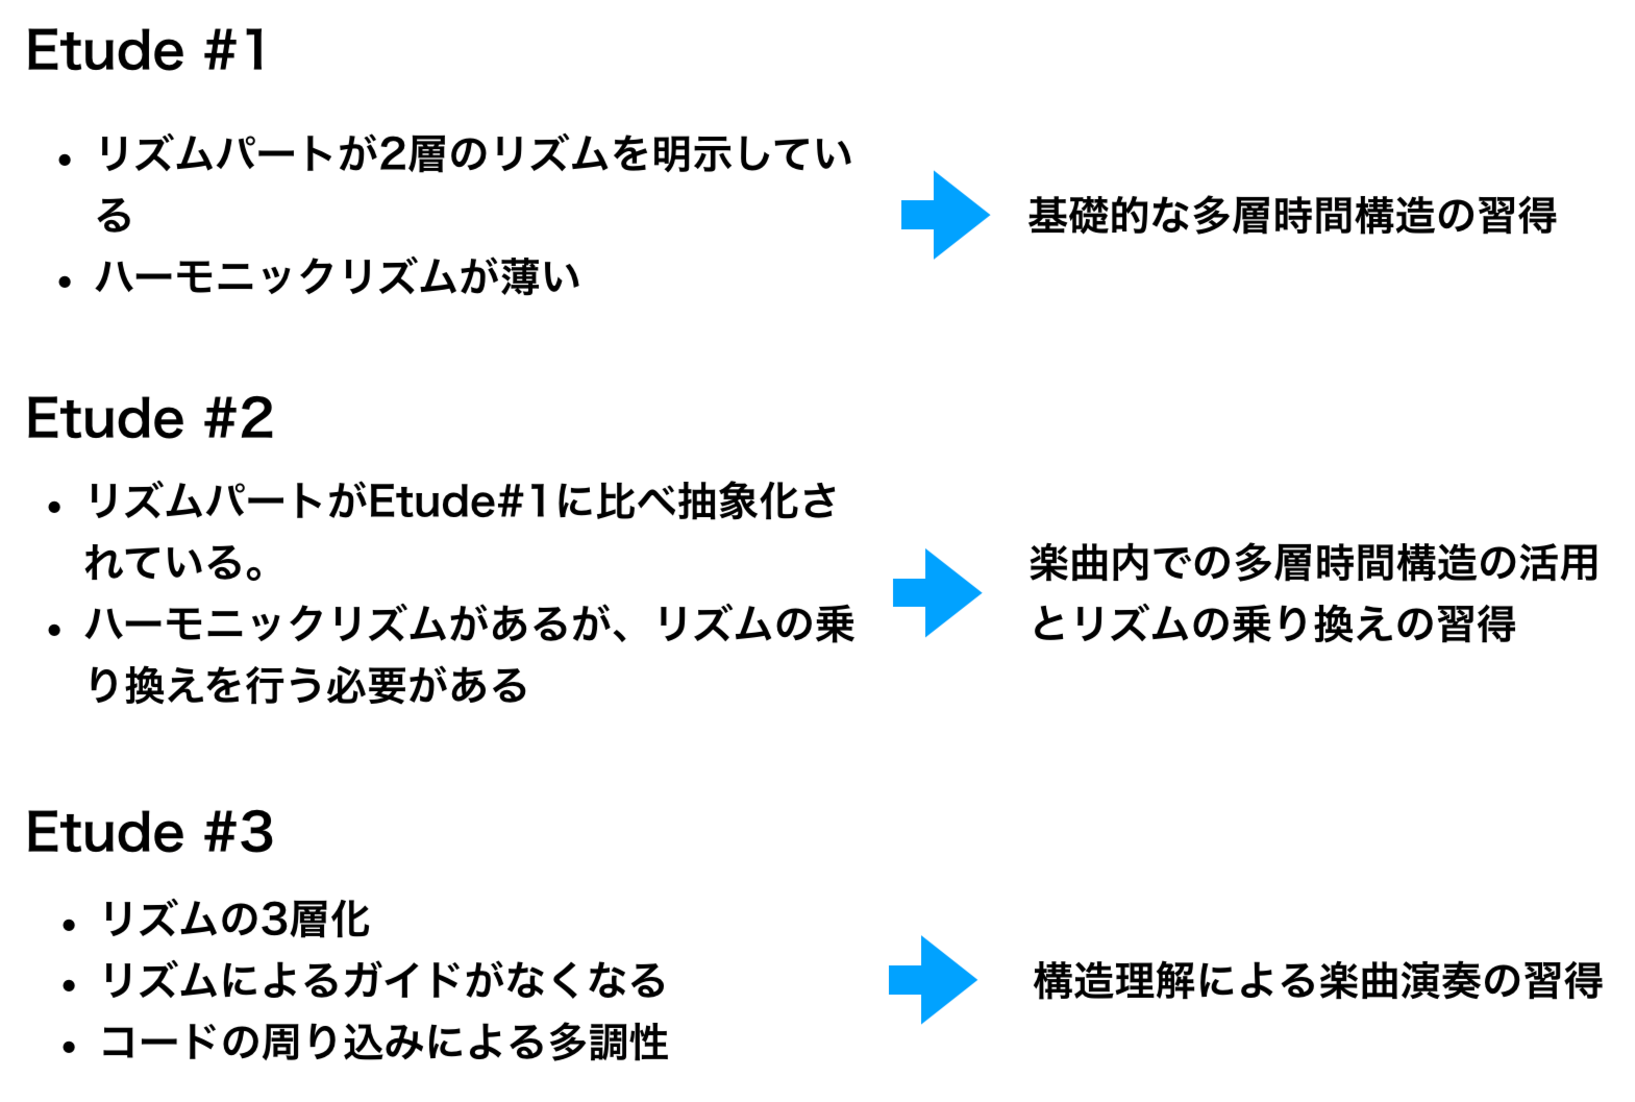
\includegraphics[
 width=\textwidth]{./PDF/figure_10.pdf}
}
\caption{Relationships between each etude}
\label{fig:figure_10}
\end{figure}

Each piece was created using Apple Logic Pro X, and simulation audio sources were produced. Each audio source can be heard at the following URLs:

\begin{enumerate}
	\item "Etude \#1" \url{https://goo.gl/Bv1odQ}
	\item "Etude \#2" \url{https://goo.gl/49g16U}
	\item "Etude \#3" \url{https://goo.gl/mzgDqu}
\end{enumerate}
